\documentclass[tikz,border=10pt]{standalone}
\usetikzlibrary{calc}
\begin{document}
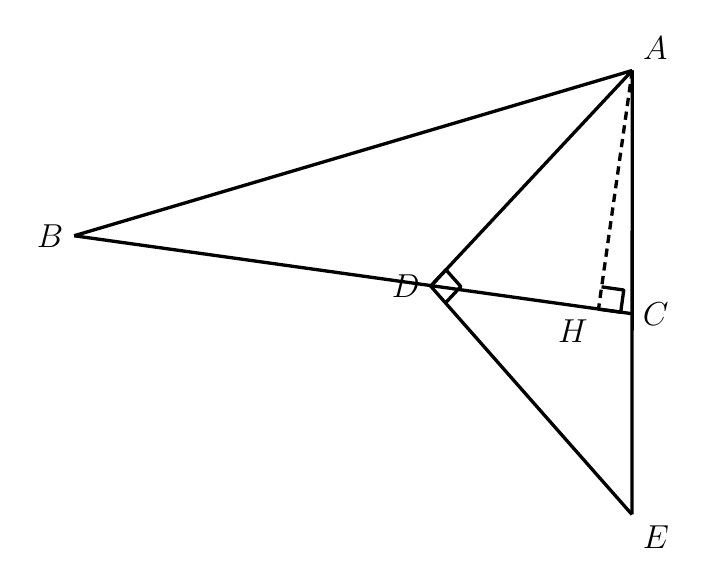
\begin{tikzpicture}[line width=1.2pt, line join=round]
% Coordinates in cm: x=(px-300)*0.014981, y=(254-py)*0.014981 (y flipped)
\coordinate (A) at (3.615,2.818);
\coordinate (B) at (-3.473,0.719);
\coordinate (C) at (3.611,-0.271);
\coordinate (D) at (1.055,0.079);
\coordinate (H) at (3.186,-0.213);
\coordinate (E) at (3.611,-2.821);

% Right-angle square at H (mark points converted from pixels)
\coordinate (P1) at (3.468,-0.252);
\coordinate (P2) at (3.507,0.030);
\coordinate (P3) at (3.225,0.070);

% Right-angle square at D for angle ADE (sides along DA and DE, 19 px)
\coordinate (Q1) at (1.249,0.287);
\coordinate (Q2) at (1.437,0.074);
\coordinate (Q3) at (1.243,-0.134);

% Solid segments
\draw (A) -- (B);          % AB
\draw (B) -- (C);          % BC, passes through D
\draw (A) -- (E);          % vertical AC E
\draw (A) -- (D);          % AD
\draw (D) -- (E);          % DE

% Dashed altitude A-H
\draw[dash pattern=on 3pt off 2pt] (A) -- (H);

% Right-angle marks at H and D
\draw (H) -- (P1) -- (P2) -- (P3);
\draw (D) -- (Q1) -- (Q2) -- (Q3);

% Labels
\node[anchor=south west, font=\fontsize{12}{14.4}\selectfont] at (A) {$A$};
\node[anchor=east, font=\fontsize{12}{14.4}\selectfont] at (B) {$B$};
\node[anchor=west, font=\fontsize{12}{14.4}\selectfont] at (C) {$C$};
\node[left, font=\fontsize{12}{14.4}\selectfont] at (D) {$D$};
\node[anchor=north east, font=\fontsize{12}{14.4}\selectfont] at (H) {$H$};
\node[anchor=north west, font=\fontsize{12}{14.4}\selectfont] at (E) {$E$};
\end{tikzpicture}
\end{document}